\chapter{Architecture et conception}

\section*{Introduction}
\addcontentsline{toc}{section}{Introduction}
\par Le troisième chapitre explore l'architecture du projet et sa étude conceptuelle. 
Nous allons justifier notre choix architectural et détaillerons la conception qui nous 
a ménné à la réalisation de notre solution.

\section{Étude architecturale}
\par  L'étude architecturale joue un rôle central dans la conception et le déploiement d'une solution robuste et évolutive.
\par Dans cette section, nous examinerons en profondeur l'architecture du système, couvrant à la fois ses dimensions logiques 
et physiques tout en discutant également les défis techniques et logiques rencontrés pour assurer une infrastructure solide et efficace.

\subsection{Architecture logique}
\par L'architecture logique constitue le fondement sur lequel repose toute la structure de notre système. Dans cette section, nous plongeons au cœur de notre étude architecturale,
 explorant les choix et les stratégies qui sous-tendent la mise en œuvre de notre solution. À travers une approche méthodique, nous détaillons les composants clés, leurs interactions et leur organisation,
  offrant ainsi une vue d'ensemble claire et précise de notre architecture logique ainsi que les patrons de conception respecter dans cette derniére.

\subsubsection{Architecture logique adoptée} 
\par Pour la mise en place de ce projet, nous avons délibérément opté pour \textbf{une architecture micro-services}, une décision dictée par des critères spécifiques qui s'accordent parfaitement avec les exigences
de notre projet ainsi que les differentes parties prenantes.
\par Cette architecture met en lumière les différents composants fonctionnels et explique comment ces composantes interagissent pour fournir une expérience utilisateur fluide et des analyses précises\cite{archi_log}. 
Cette derniére est illustrée par la figure \textbf{\ref{fig :arch_log}} suivante  :
%code image
        \begin{figure}[H]
        \centering
        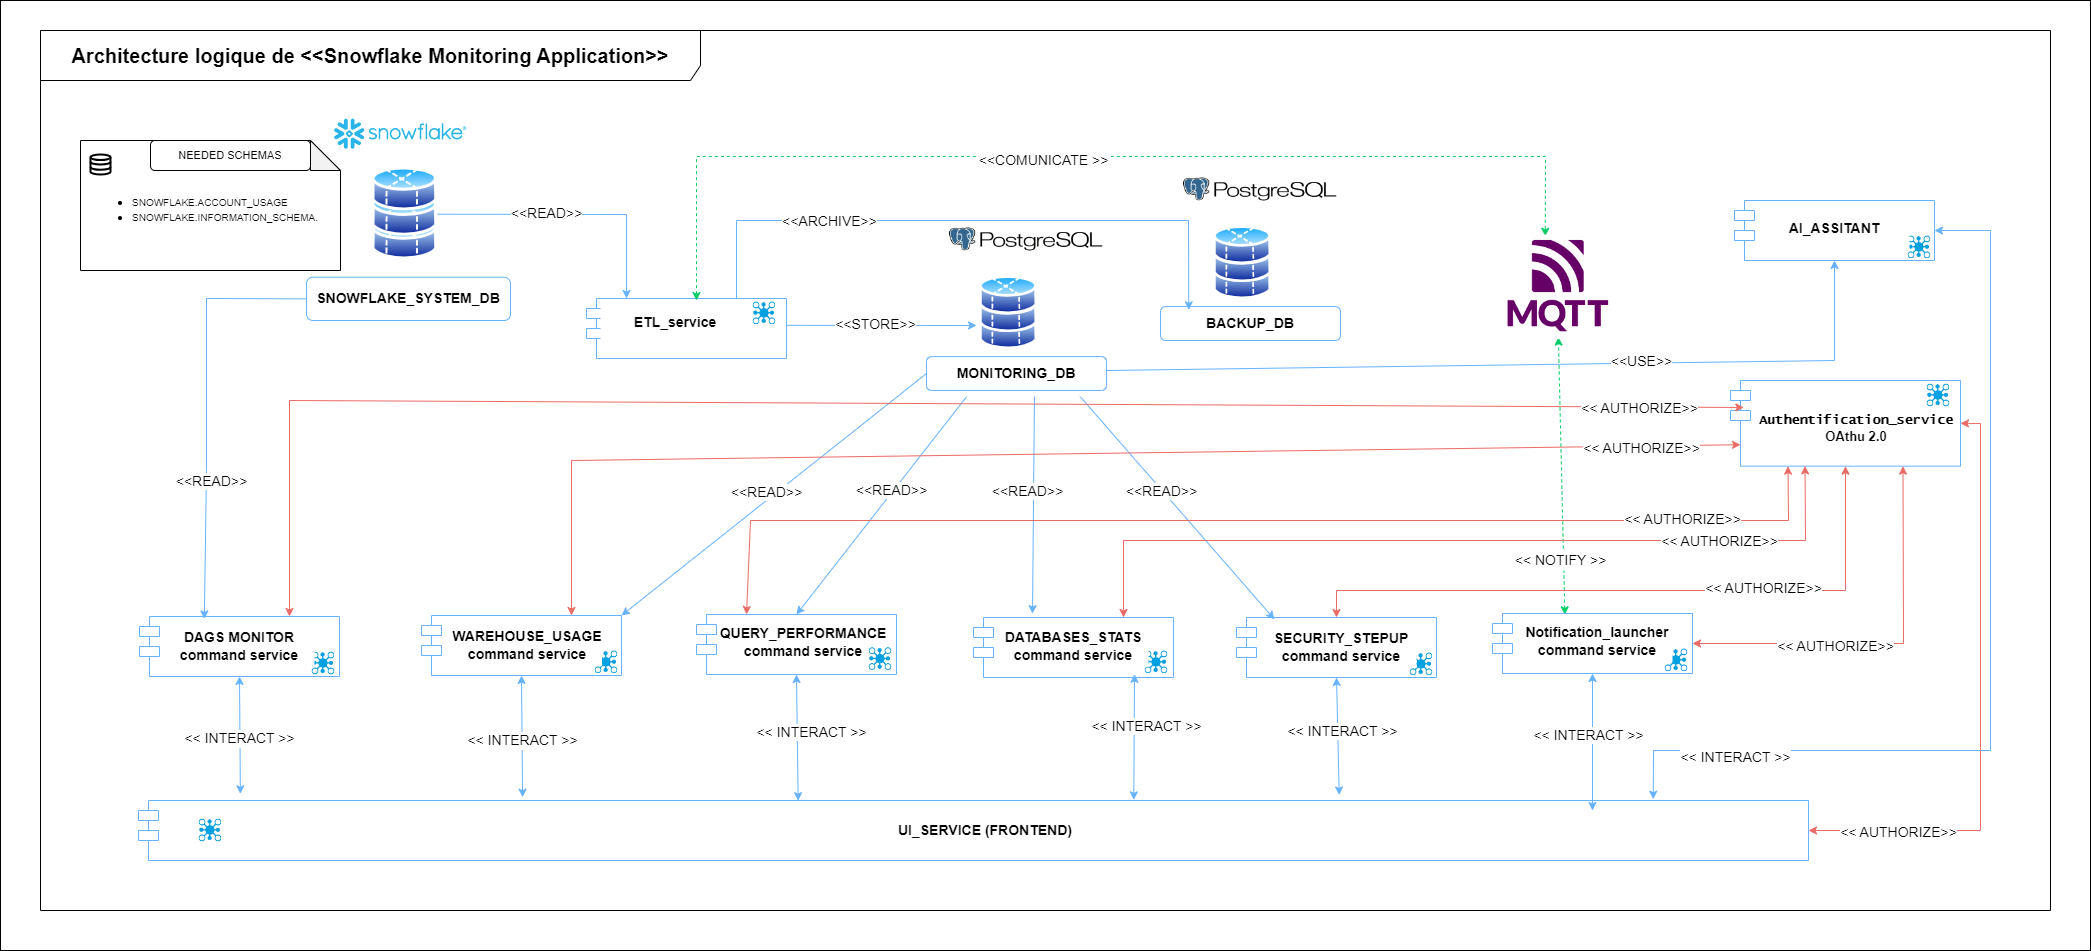
\includegraphics[width = 1\linewidth]{img/conception/archi.png}
        \caption{Architecture logique de <<Snowflake Monitoring Application>>}
    \label{fig :arch_log}
        \end{figure}
        %fin
    \par Notre architecture est repartie comme suit : 
    \begin{enumerate}

        \item[1.] \textbf{Couche des données :} 
                \begin{itemize}
                \item \textbf{Snowflake} : ce composant représente les vues sytémes de Snowflake telque <<Account\_ussage>> et <<information\_schema>> qui regroupent tous les données à monitorer ;
                %\item \textbf{Monitoring_DB_Snowflake} : elle garantit une transformation et une intégration harmonieuse des données pour une analyse ultérieure.
                \item \textbf{Monitoring\_DB} : c'est une base de données PostgreSQL stockant les données de monitoring collectées ;
                \item \textbf{BACKUP\_DB} : c'est une base de données PostgreSQL utilisée pour l'archivage des données, qui permet de garantir la durabilité et la redondance des données, en cas de panne ou de besoin de restauration des données de MONITORING\_DB principale.

            \end{itemize}
            
         \item[2.] \textbf{Couche applicative << micro-services >> :}
                \begin{itemize}
                \item \textbf{Etl\_Service} : service responsable de l'extraction, la transformation et du chargement des données de la platforme Snowflake vers la base de données de monitoring ;
                \item \textbf{DAG\_Monitoring} : service responsable du suivi et de la surveillance des flux de tâches programmées dans Snowflake en temps réelle (<<DAG>>) ;
                \item \textbf{Warehouse\_Monitoring} : service chargé de la surveillance de l'utilisation, créditation et toutes informations concernant les entrepôts de données Snowflake ;
                \item \textbf{Query\_Performance } : service d'analyse, collecte et traitement des performances des requêtes Snowflake ;
                \item \textbf{ Databases\_Statistics} : service d'analyse, collecte et traitement des statistiques sur les bases de données Snowflake ;
                \item \textbf{Access\_Statistics} : service d'analyse, collecte et traitement des statistiques sur les access des utilisateurs des différents comptes et entrepôts de données Snowflake ;
                \item \textbf{Notifications\_Launcher } :service responsable de la gestion des notifications, il se charge de transmettre les notifications reçus aux utilisateurs finaux par les canaux de communication appropriés ;
                \item \textbf{Authentification\_Service } : service d'authentification et d'autorisation basé sur OAuth 2.0 ;
                \item \textbf{AI\_ASSISTANT\_service } : service d'assistance IA intégré dans l'architecture pour apporter une dimension d'intelligence artificielle aux fonctionnalités de surveillance, d'analyse et d'optimisation des requêtes SQL.

            \end{itemize}
                \par Cette couche assure la gestion de la logique métier de l'application en traitant et examinant les données collectées.
                Elle interagit avec l'interface utilisateur pour fournir des informations et des résultats pertinentes.
        \item[3.] \textbf{Couche de Communication : }
                \begin{itemize}
                    \item \textbf{MQTT} : système de messagerie basé sur le protocole MQTT, utilisé pour la communication asynchrone et découplée entre les différents services ;
                    \item \textbf{MQTT Broker} : composant central du système MQTT, chargé de la distribution des événements publiés par les services ;
                    \item \textbf{REST} : la communication entre les microservices ce fait via des APIs REST.
                \end{itemize}
            
        \item[4.] \textbf{Couche de Présentation  :}
            \begin{itemize}
                \item \textbf{UI\_Service} : ce servise fournit des tableaux de bord et des interfaces utilisateur pour visualiser les données de monitoring.
                \par Il offre une expérience utilisateur conviviale et interactive pour la visualisation des données de performance et les résultats d'analyse.
            \end{itemize}
    \end{enumerate}
    \par En conclusion, l'architecture logique adoptée, basée sur une approche micro-services, divise notre système en composants modulaires interagissant de manière fluide pour garantir la fonctionnalité globale de l'application. 
    Cette approche assure une gestion efficace des données, une scalabilité optimale et une expérience utilisateur conviviale, constituant ainsi le fondement solide de notre solution de gestion et d'analyse de données.
\subsubsection{Justification du choix de l'architecture micro-services}

\par Le choix de l'architecture d'une application revêt une importance capitale dans le processus de conception d'un projet. 
Il détermine comment les diverses parties de l'application interagissent pour atteindre les objectifs fixés.
\par Dans cette section, nous explorerons en détail les raisons pour lesquelles nous avons opté pour cette architecture, en soulignant sa pertinence pour notre projet.
\begin{itemize}
        \item \textbf{Flexibilité et scalabilité : } nous avons choisi l'architecture microservices pour sa flexibilité et sa capacité à évoluer facilement. 
        Car, chaque service fonctionne de manière indépendante, ce qui permet une adaptation aisée aux évolutions du système. Cette approche modulaire offre la possibilité 
        d'ajouter de nouveaux services ou de mettre à l'échelle les services existants en fonction des besoins croissants de l'application ; \\ 

        \item \textbf{Modularité et maintenance : } la modularité est au cœur de l'architecture microservices, offrant un avantage significatif en termes de maintenance.
        En effet, chaque service peut être développé, testé et déployé de manière autonome, ce qui facilite la gestion des mises à jour et des correctifs, tout en isolant 
        les composants fonctionnels du système, cette approche permet de limiter l'impact des changements sur l'ensemble de l'application.
         Assurant ainsi une maintenance plus efficace et moins sujette aux erreurs ;\\

        \item \textbf{Réutilisabilité et flexibilité technologique :} grâce à l'approche par microservices, notre projet bénéficie d'une grande réutilisabilité du code et
         d'une flexibilité technologique accrue. De fait, chaque service peut être développé en utilisant les technologies les mieux adaptées à ses besoins spécifiques, ce qui favorise 
         l'adoption des meilleures pratiques et des outils les plus performants pour chaque composant. Car ette modularité permet également de réutiliser efficacement les services
          existants dans d'autres projets ou contextes, ce qui contribue à une meilleure efficacité du développement logiciel ; \\


         \item \textbf{Évolutivité et résilience :} les microservices favorisent une architecture résiliente et évolutive. 
         En cas de panne d'un service, les autres services peuvent continuer à fonctionner normalement, ce qui réduit les interruptions.
         De plus, cette approche permet une meilleure répartition de la charge, assurant des performances optimales même lors de pics de trafic.
\end{itemize}
\par En conclusion, l'adoption de l'architecture microservices se révèle être un choix judicieux pour notre projet, offrant une solution flexible, modulaire et résiliente.
Elle nous permet de répondre efficacement aux besoins changeants de nos utilisateurs tout en garantissant des performances et une fiabilité optimales.
\subsubsection{Patrons de conception}
\par Les patrons de conception représentent des solutions éprouvées à des problèmes fréquents en conception logicielle. Ce sont comme des modèles ou des structures que l'on peut adapter pour résoudre des problèmes récurrents dans notre code\cite{design_pattern}.
\par Lors de l'élaboration de cette architecture, nous avons focaliser sur le fait de respecter les patrons de conception afin d'avoir une architecture solide et structurée.
\par Nous avons utilisé les patrons de conception suivants :
\begin{itemize}
    \item \textbf{Le patron <<Command Query Responsibility Segregation (CQRS)>>} : il est aussi un model d'architecture qui sépare les deux parties de traitement (Écriture) et de réponse (Lecture) \cite{CQRS}.
    \par L'architecture applique le modèle CQRS, avec une séparation des responsabilités entre le services de commande (ETL\_service) et les services de requête (tout les autres services).
    Cette séparation optimise les performances des flux de lecture et d'écriture de manière indépendante ; \\
    \item \textbf{Le patron <<Façade>>} : c'est un modèle de conception structurel qui fournit une interface simplifiée pour accéder à une bibliothèque, 
    un framework ou à tout ensemble complexe de classes\cite{facade}.
    \par Le service <<ETL\_service>> fait office de façade, en encapsulant la complexité de l'interaction avec Snowflake, 
    de façon que les autres services n'ont pas besoin de connaître les détails de l'interaction avec Snowflake ; \\
    \item \textbf{Le patron <<Observateur>>} : c'est un modèle de conception comportemental qui permet d'établir un mécanisme de souscription pour envoyer des notifications à plusieurs objets concernant des événements liés aux objets qu'ils observent\cite{observer}.
    \par Le service <<MQTT\_broker>> fait office d'observateur, car implémente un modèle de publication/souscription, permettant aux services de s'abonner aux événements qui les intéressent.
    Cela découple les services et facilite l'ajout de nouveaux services.
    \item \textbf{Le principe <<de responsabilité unique (SRP)>>} : ce principe dénance que chaque qu'un composant (classe, service, module, etc.) ne doit avoir qu'une seule raison de changer. 
    Cela se traduit par une séparation claire des responsabilités au sein de l'architecture\cite{SRP}.
    \par Chaque microservice (DAGS\ MONITOR, WAREHOUSE\_USAGE, QUERY\_PERFORMANCE, etc.) est responsable d'une fonctionnalité spécifique du monitoring.
   \par De plus, la séparation entre la base de données Snowflake (données surveiller) et la base de données Monitoring\_DB (données de monitoring) respecte le SRP ; \\
    \item \textbf{Le patron <<Objet d'accès aux données (DAO)>>} : ce moàdéle représente une façon d'organiser le code pour gérer la communication entre le programme et la base de données.
    Il permet de conserver un code propre et de séparer la logique d'interaction avec les données du reste de l'application\cite{DAO}.
    \par L'accès à la base de données de monitoring (Monitoring\_DB) est géré via un modèle DAO, séparant la logique d'accès aux données du reste de l'application.
    Cela améliore la maintenabilité et permet une indépendance entre la couche de données et la logique métier.
\end{itemize}
\par En conclusion, l'architecture logique adoptée, basée sur des microservices, offre une approche modulaire et flexible, permettant une gestion efficace des données et une évolutivité optimale de l'application. En intégrant des patrons de conception pertinents,
 nous garantissons une structure robuste et cohérente, répondant aux exigences spécifiques de notre projet de surveillance et d'analyse des données.
\subsection{Architecture physique}
    \par L'architecture physique d'un projet constitue la matérialisation concrète de son architecture logique. Elle se consacre aux aspects matériels et aux ressources nécessaires pour assurer le bon fonctionnement de l'application\cite{archi_phy}.
    \par Pour la mise en place de cette solution de monitoring Snowflake, nous avons suivi une approche en n-tiers afin de garantir une séparation claire des responsabilités, 
    une meilleure évolutivité et une plus grande résilience de l'ensemble du système. 
    Elle permet une gestion efficace des ressources, une répartition optimale des charges de travail et une sécurisation renforcée de l'infrastructure. 
    \par La figure \textbf{\ref{fig :arch_phy}} suivante illustre l'architecture adopté dans ce projet  : 
%code image
        \begin{figure}[H]
        \centering
        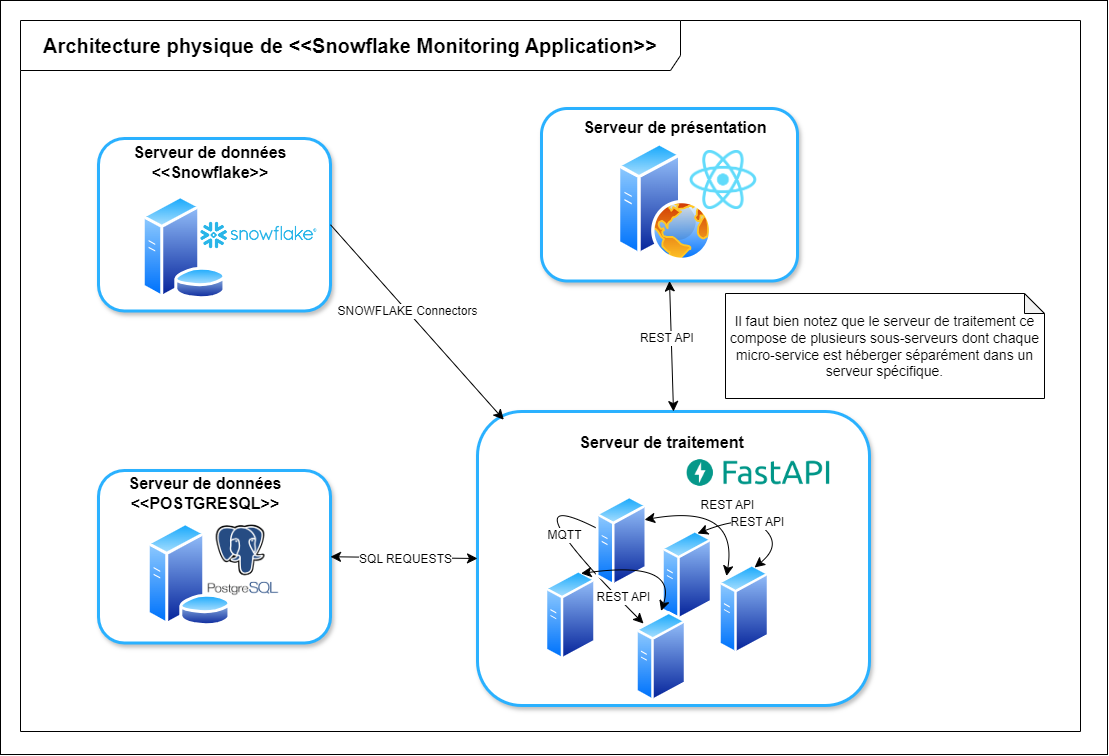
\includegraphics[width = 17cm ]{img/conception/archi_phy.png}
        \caption{Architecture physique de <<Snowflake Monitoring Application>>}
        \label{fig :arch_phy}
        \end{figure}
        %fin
        \par Notre architecture physique est composée de plusieurs éléments essentiels qui travaillent cycliquement pour permettre la collecte, le traitement, le stockage et la présentation des données de manière optimale. Voici un aperçu détaillé de ces composants  :
        \begin{enumerate}
            \item[1-] \textbf{Tier des Services (Tier Application) : } 
            cet tier comprend les différents serveurs d'application hébergeant les microservices du système.
            \par Il inclut des serveurs pour les services DAGS\_MONITOR, WAREHOUSE\_USAGE, QUERY\_PERFORMANCE, ETL\_service, AUTH\_service, etc.
            \par Ces serveurs sont responsables de la logique métier et du traitement des données ;
            \item [2-] \textbf{Tier des Données :} 
            cet tier est composé du serveur de base de données hébergeant la base de données MONITORING\_DB.
            \par Il est chargé du stockage et de la gestion des données de monitoring collectées.
            \par Le serveur Snowflake, hébergeant la base de données SNOWFLAKE\_SYSTEM\_DB, fait également partie de ce tier des données ;
             
            \item[3-]  \textbf{Tier de présentation : }
            cet tier comprend le serveur frontend hébergeant le service ui\_service.
            \par Il est responsable de la présentation des données de monitoring aux utilisateurs via les tableaux de bord et les interfaces ;
            \item[4-] \textbf{inter-communication :}
            cet tier représente les modes de communication utilisés entre les composants de l'architecture, via les requêtes SQL, les API REST, les connecteurs Snowflake et le système de messagerie MQTT.

        \end{enumerate}
    \par Cette architecture en n-tiers offre plusieurs avantages clés, tels que la séparation des préoccupations, l'évolutivité, la résilience et la sécurité renforcée du système. 
    Chaque tier étant responsable d'une fonction spécifique, il devient plus aisé de maintenir, de mettre à l'échelle et de sécuriser les différents composants de manière indépendante.
\section{Étude conceptuelle}
\par Dans cette section, nous allons s'intéresser à la modélisation de notre projet à l'aide des différents modelés et diagrammes qui vont nous permettre de mieux
 comprendre le flux de travail ainsi la nature des données et les traitements qui circulent dans notre système.
\subsection{Conception globale}
    \par Dans cette section, nous allons illustrer les differents diagrammes modélisant la conception globale de notre solution.
    \subsubsection{Diagramme de paquetages}
    \par Les diagrammes de paquetages sont des diagrammes structurels qui illustrent l'organisation et la disposition de différents éléments modélisés sous forme de packages\cite{diag_pack}.

    \par Il sert à grouper des éléments en un ensemble cohérent, et à fournir un espace de noms pour ces éléments.\par La figure \textbf{\ref{fig :pack}} qui suit représente le diagramme de paquetages de notre système : 
        %code image
            \begin{figure}[H]
            \centering
            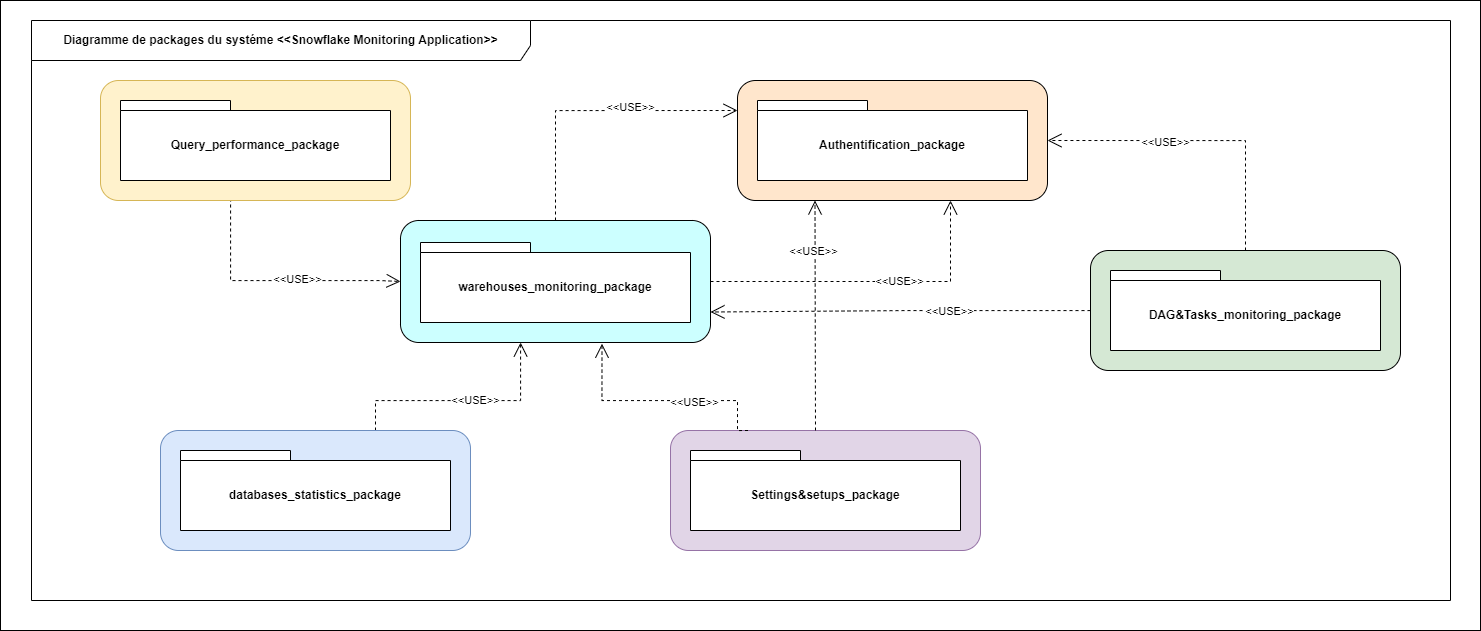
\includegraphics[width=1\linewidth]{img/conception/diag_pack.png}
            \caption{Diagramme de paquetages de <<Snowflake Monitoring Application>>}
            \label{fig :pack}
            \end{figure}
        %fin
    \subsubsection{Diagramme de classe}
        \par Les diagrammes de classes fournissent une représentation détaillée de la structure d'un système spécifique.
        Ils modélisent les classes du système, leurs attributs, leurs opérations ainsi que les relations entre les objets\cite{diag_class}. 
        \par Ce diagramme permet de visualiser clairement la composition du système, facilitant ainsi la compréhension des interactions et des dépendances entre les différents éléments. 
        En représentant les attributs et les méthodes des classes, ils aident également à définir les responsabilités et les comportements des objets dans le contexte global du système.
        \par Dans cette partie, nous allons lister le diagrammes de classe de chaque package.
        \begin{itemize}
            \item\textbf{Packages <<Authentification>> et <<Notification>>} : la figure \textbf{\ref{fig :class1}} qui suit représente le diagramme de classe des deux packages \textbf{<<authentification>>} et \textbf{<<Notification>>} : 
        %code image
            \begin{figure}[H]
                \centering
                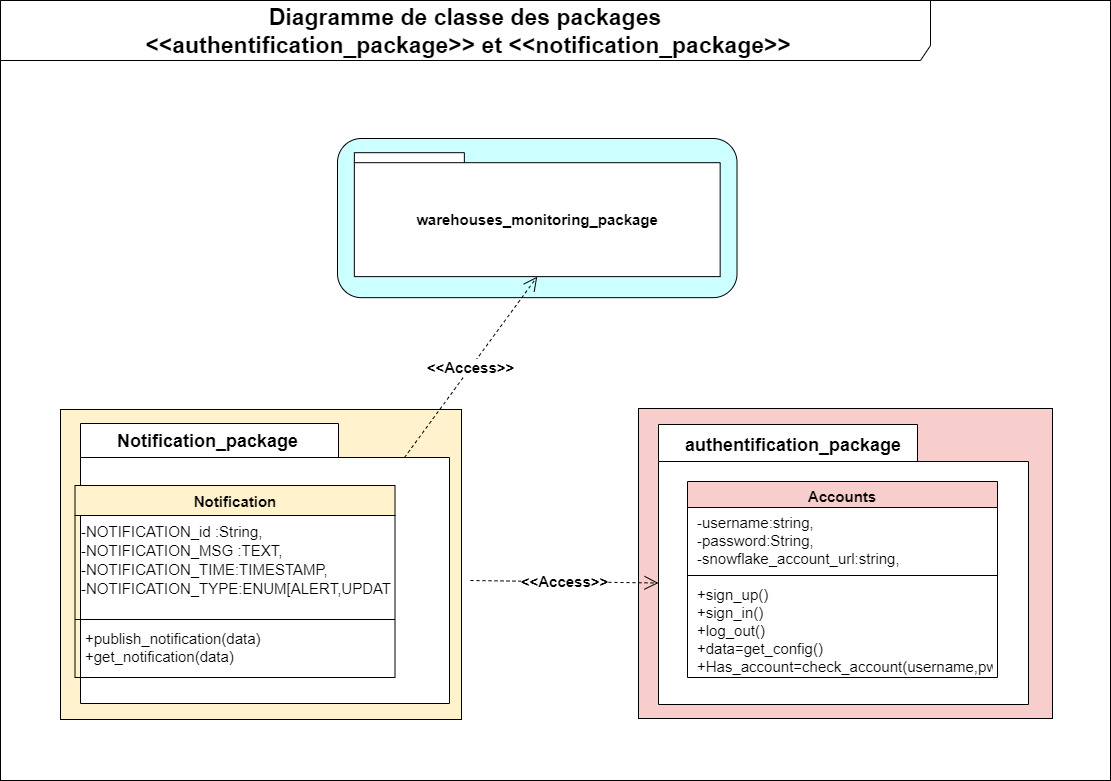
\includegraphics[width =0.8\linewidth , height =8cm]{img/conception/class_auth_notif.png}
                \caption{le diagramme de classe des deux packages <<authentification>> et <<Notification>>}
                \label{fig :class1}
                \end{figure}
        %fin
            \item\textbf{Package <<Warehouse\_monitoring>>} : la figure \textbf{\ref{fig :class2}} qui suit représente le diagramme de classe du package \textbf{<<Warehouse\_monitoring>>} : 
            %code image
            \begin{figure}[H]
                \centering
                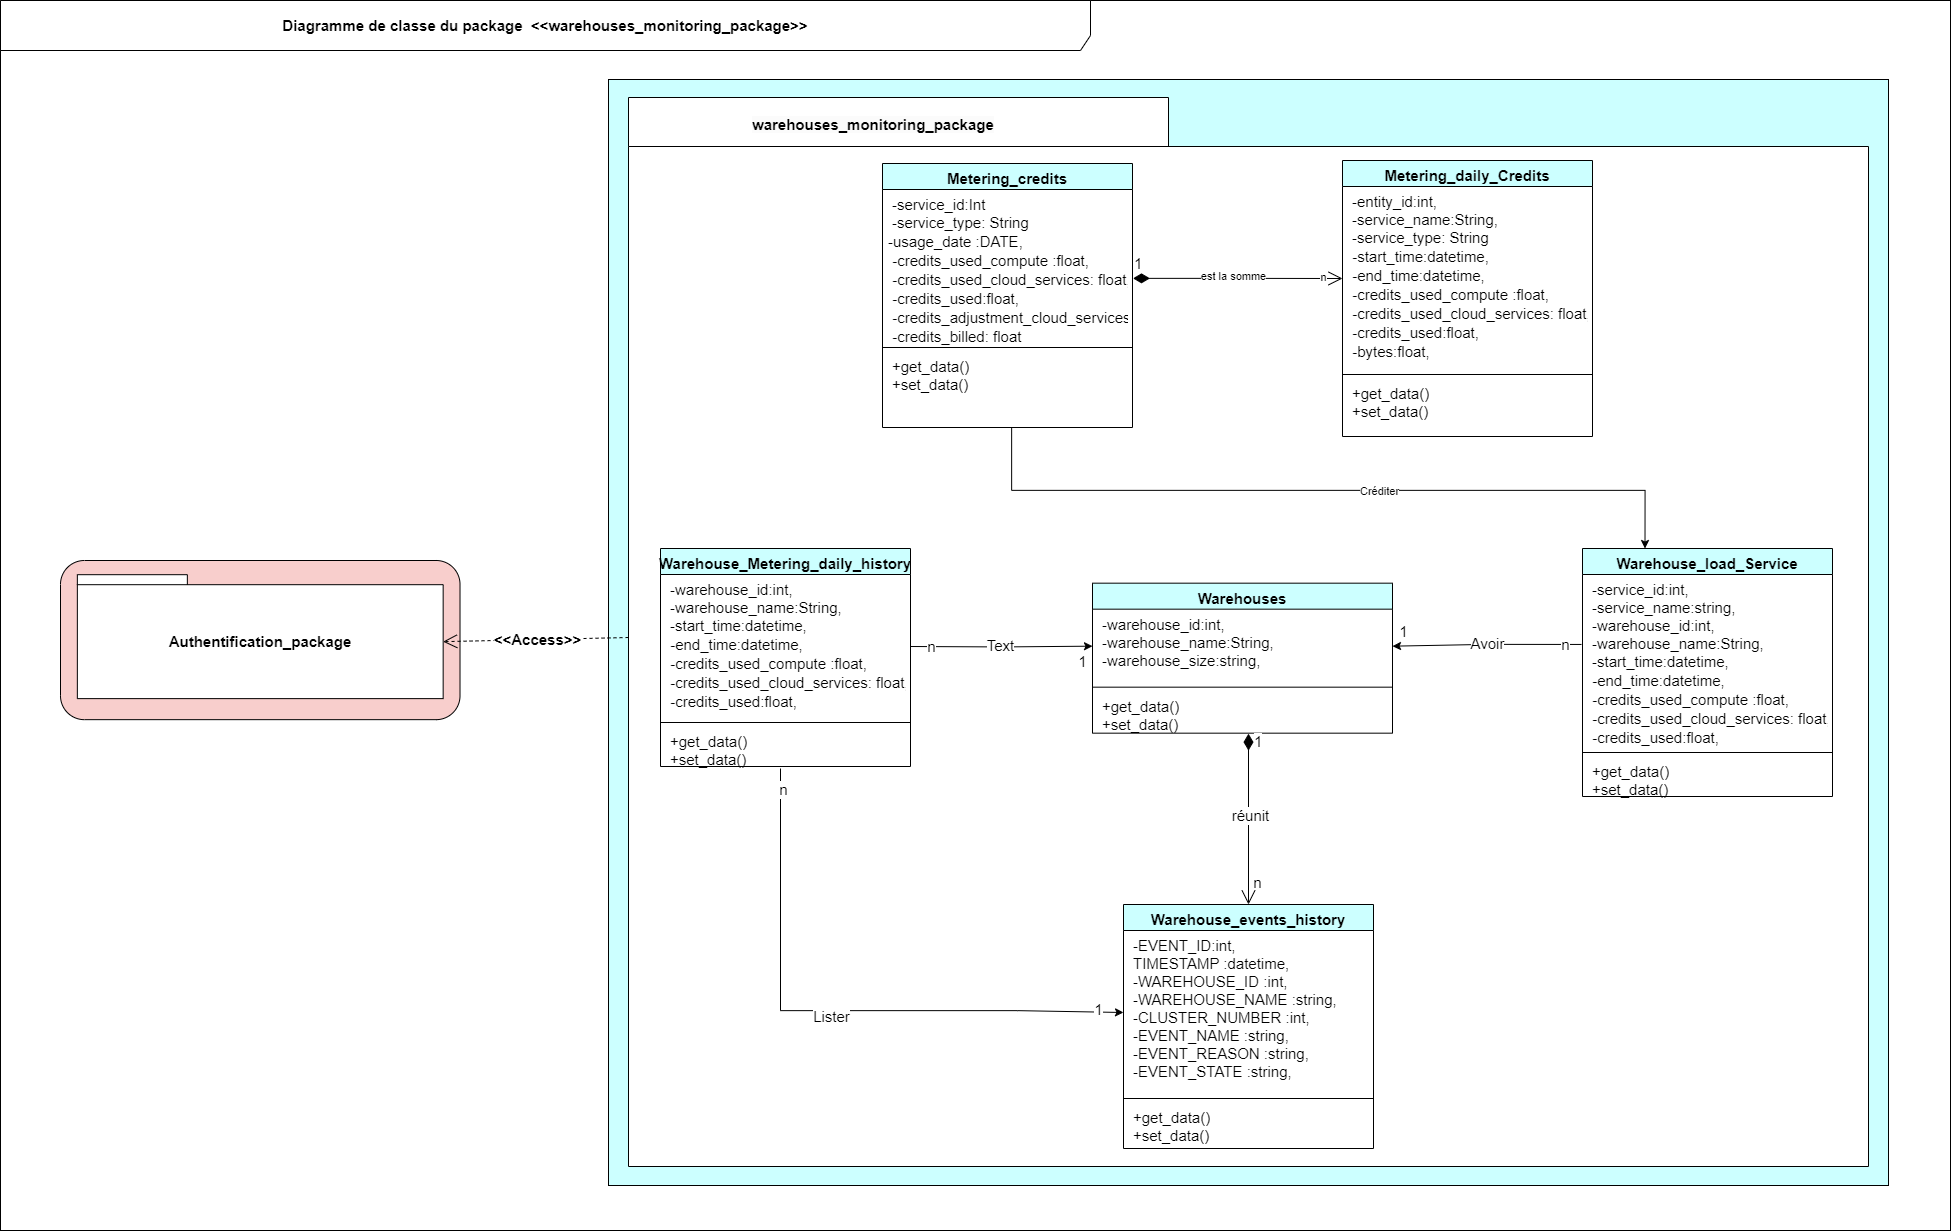
\includegraphics[width =0.8\linewidth]{img/conception/class_warehouse.png}
                \caption{le diagramme de classe du package <<Warehouse\_monitoring>>}
                \label{fig :class2}
                \end{figure}
            \newpage
                \item\textbf{Package <<Dag\&tasks>>} : la figure \textbf{\ref{fig :class3}} qui suit représente le diagramme de classe du package \textbf{<<Dag\&tasks>>} : 
            %code image
            \begin{figure}[H]
                \centering
                \includegraphics[width =0.8\linewidth,height=7cm]{img/conception/class_dag.png}
                \caption{le diagramme de classe du package <<Dag\&tasks>>}
                \label{fig :class3}
                \end{figure}
                \item\textbf{Package <<Databases\_statistics>>} : la figure \textbf{\ref{fig :class4}} qui suit représente le diagramme de classe du package \textbf{<<Databases\_statistics>>} : 
            %code image
            \begin{figure}[H]
                \centering
                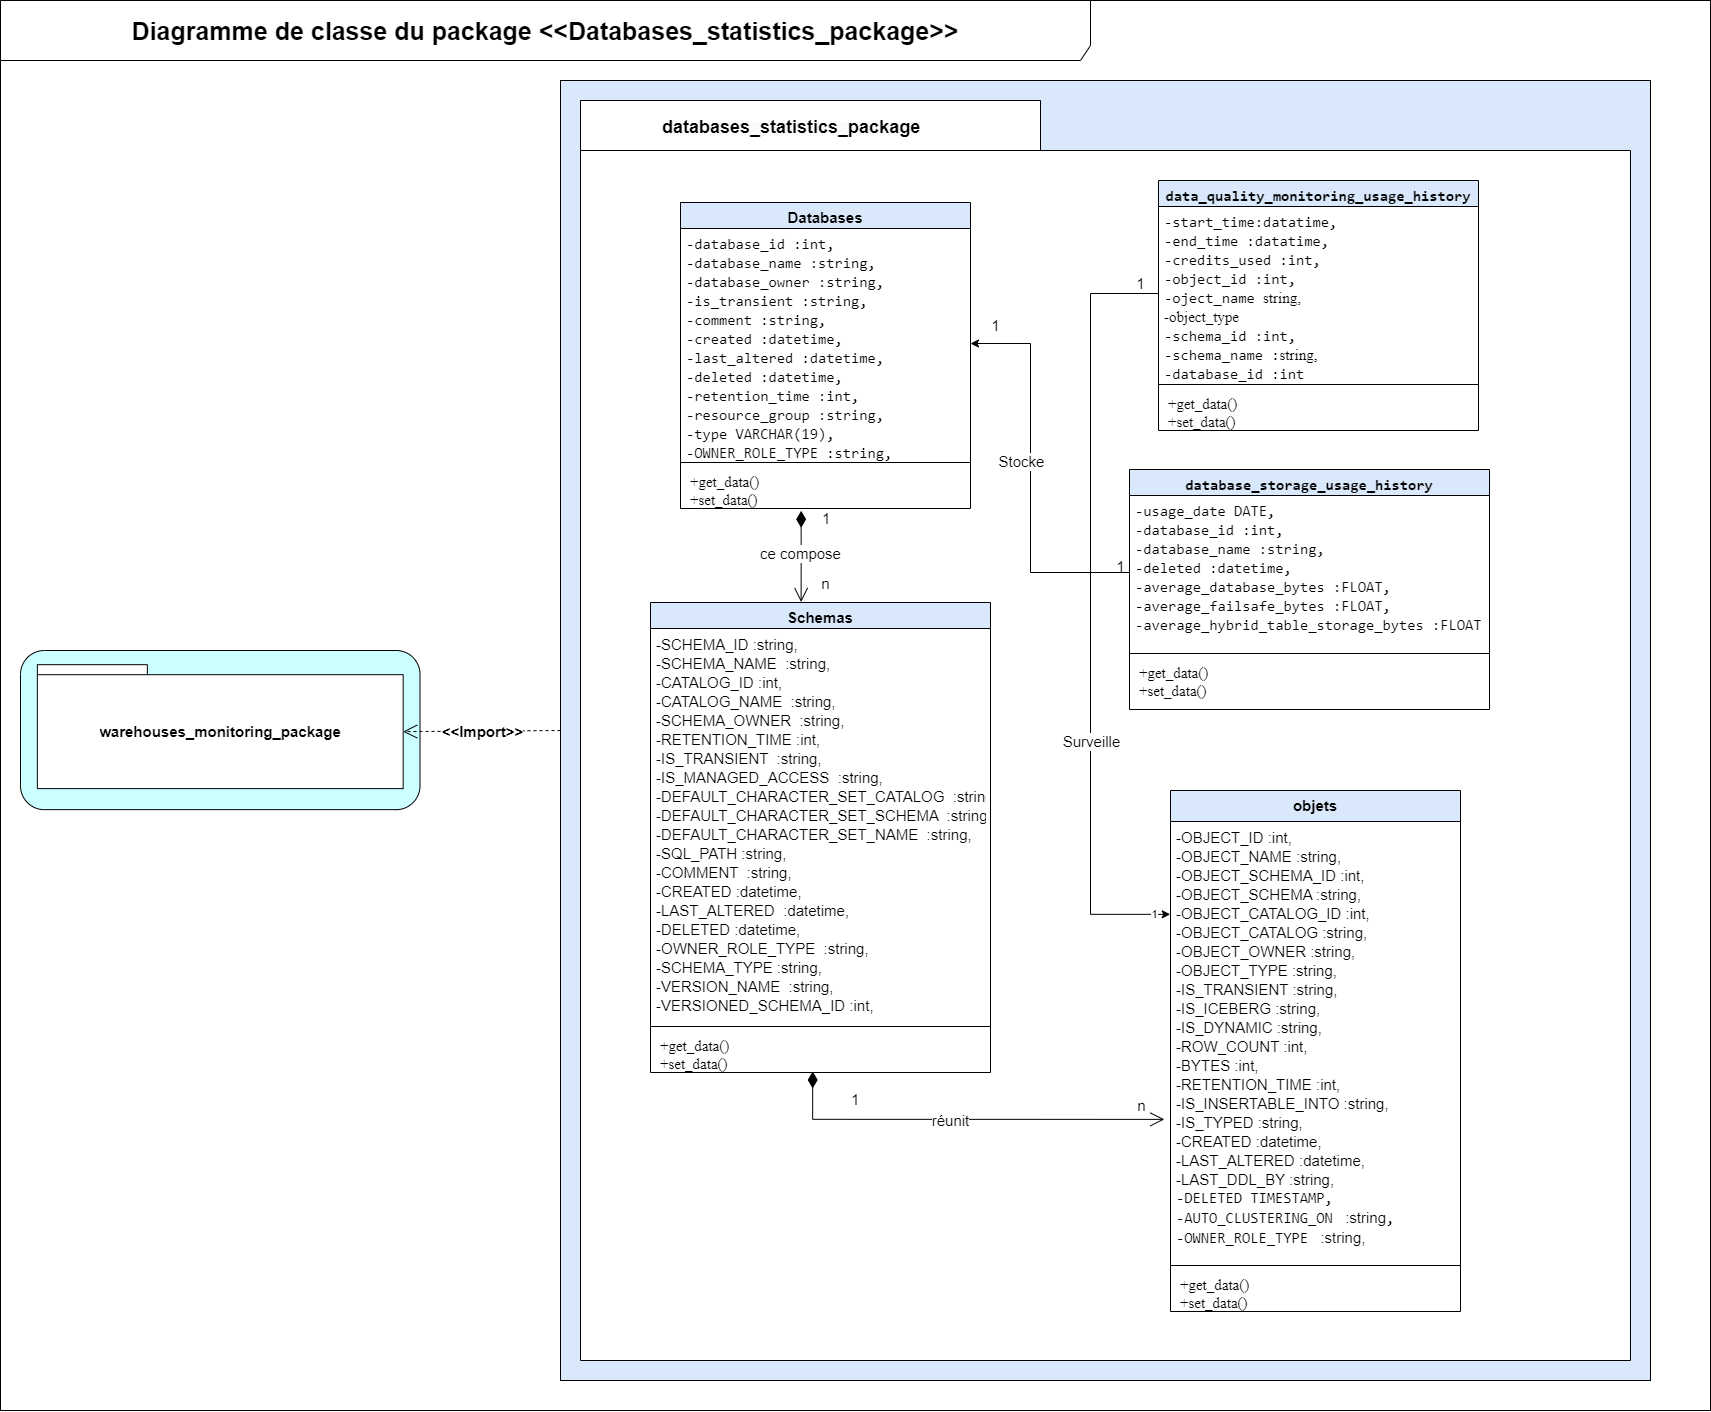
\includegraphics[width =0.8\linewidth,height=12cm]{img/conception/class_database.png}
                \caption{le diagramme de classe du package <<Databases\_statistics>>}
                \label{fig :class4}
                \end{figure}
                \item\textbf{Package <<Users\_access>>} : la figure \textbf{\ref{fig :class5}} qui suit représente le diagramme de classe du package \textbf{<<Users\_access>>} : 
            %code image
            \begin{figure}[H]
                \centering
                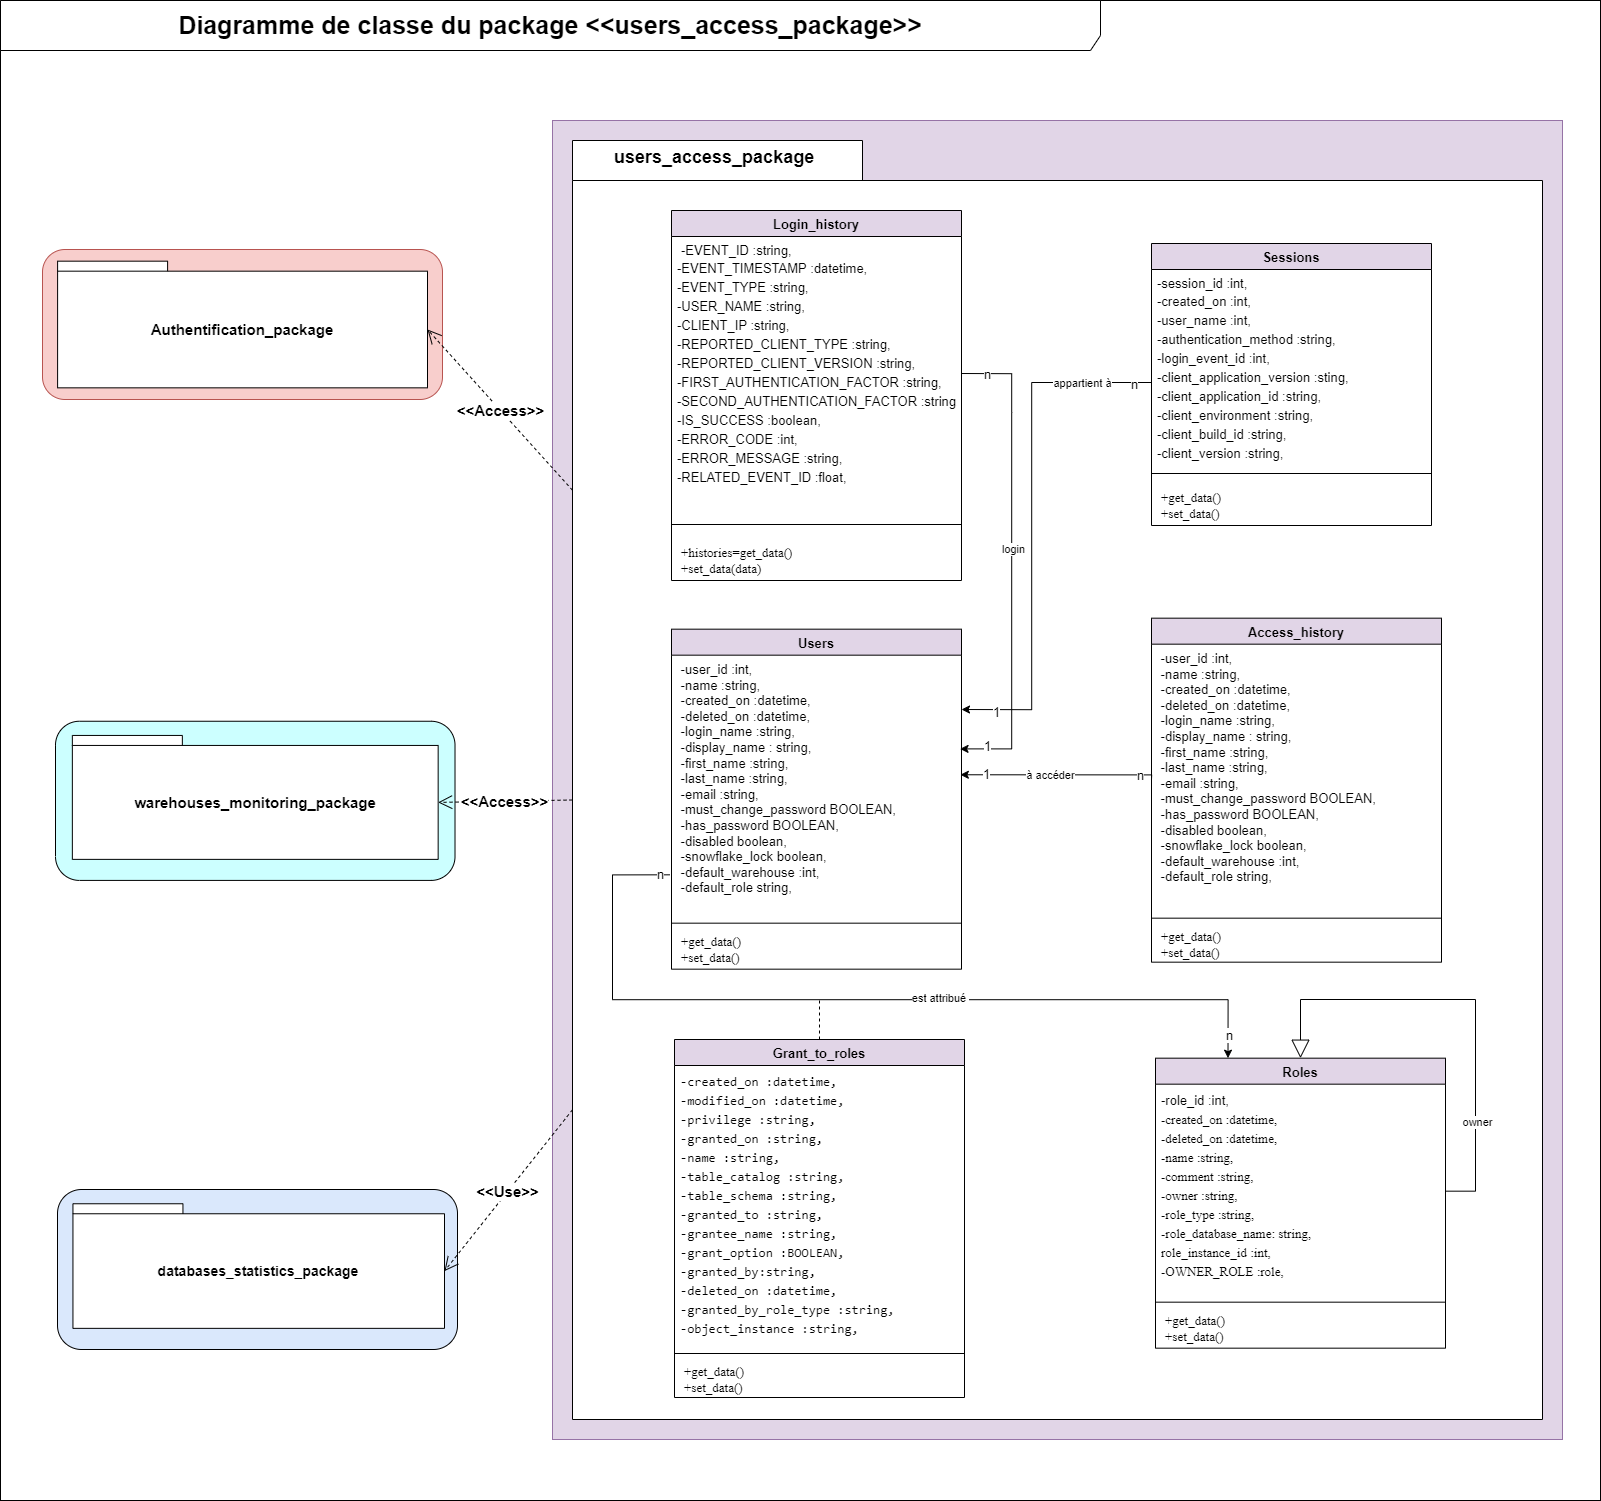
\includegraphics[width =0.8\linewidth , height=11cm]{img/conception/class_access.png}
                \caption{le diagramme de classe du package <<Users\_access>>}
                \label{fig :class5}
                \end{figure}
                \item\textbf{Package <<Query\_performance>>} : la figure \textbf{\ref{fig :class6}} qui suit représente le diagramme de classe du package \textbf{<<Query\_performance>>} : 
            %code image
                \begin{figure}[H]
                \centering
                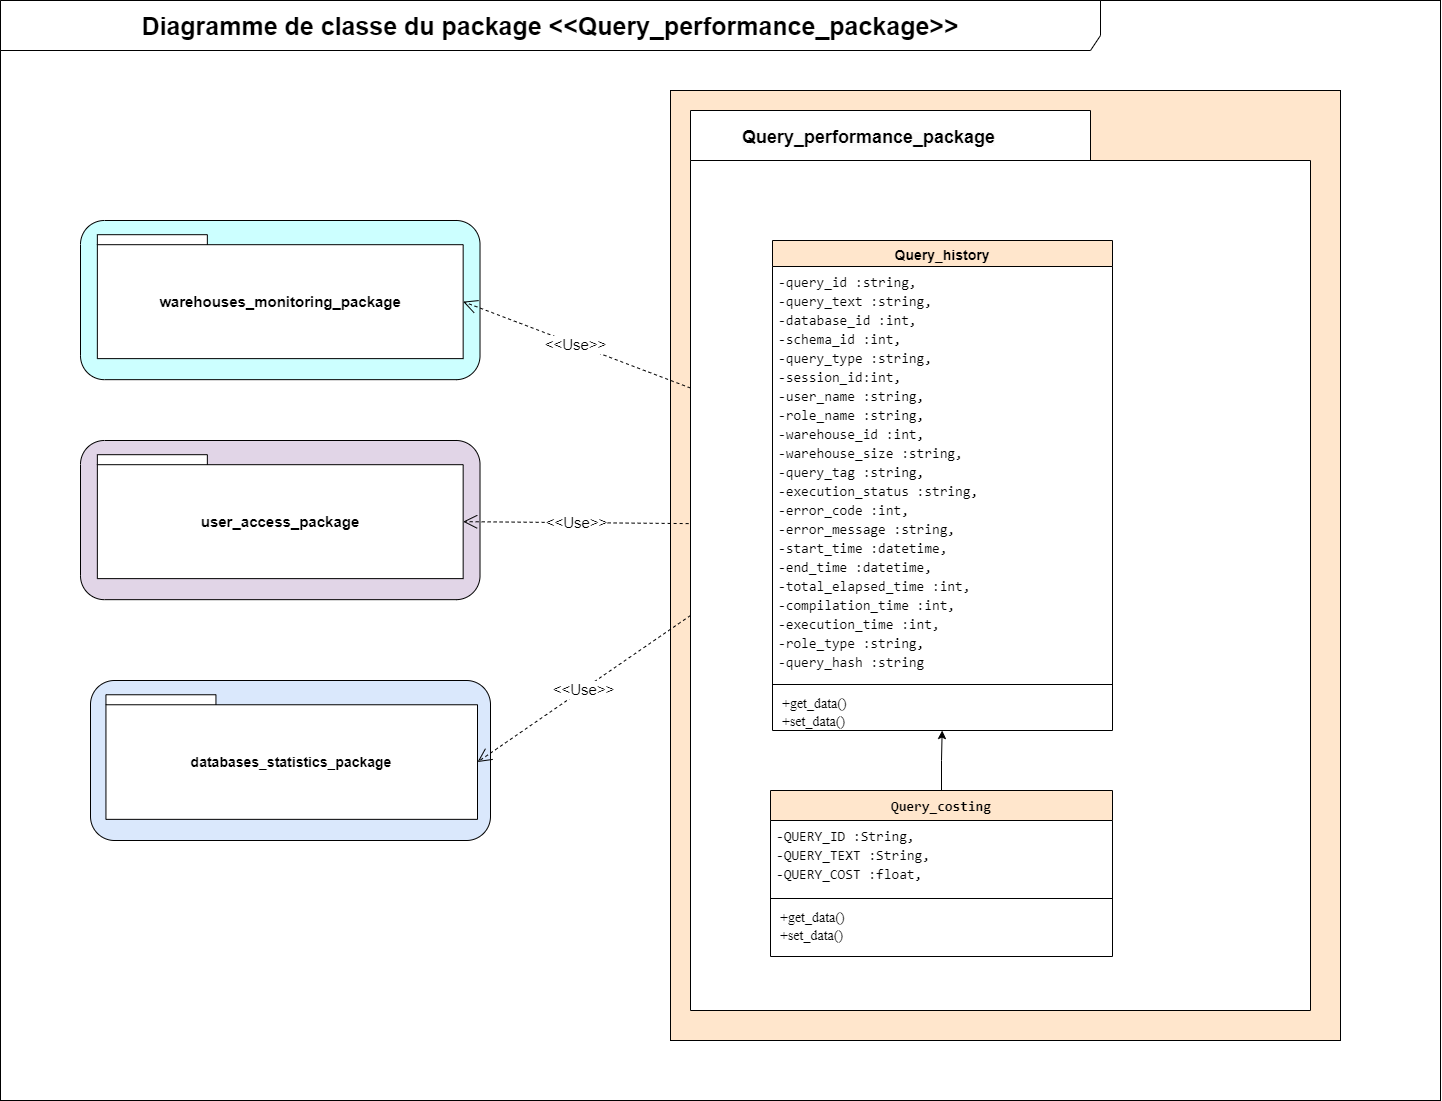
\includegraphics[width =0.8\linewidth , height=8cm]{img/conception/class_query.png}
                \caption{le diagramme de classe du package <<Query\_performance>>}
                \label{fig :class6}
                \end{figure}
            %fin
        \end{itemize}
        
        %fin
\subsection{Conception detaillée}
\par Dans cette section, nous allons s'intéresser à présenter les diagrammes illustant la conception détaillée de chaque micro-service présent dans solution.
\subsubsection{Description textuelle des cas d'utilisation}
\par c'est une description claire et précise des interactions entre les acteurs et le système pour mener à bien le cas d'utilisation. Cette description identifie les acteurs impliqués ainsi que les autres cas d'utilisation pertinents\cite{descp}.
\begin{enumerate}
    \item[1.] \textbf{Description textuelle du cas d'utilisation <<Lister les entrepôts de données>> :}
    \begin{table}[H]
        \centering
            \begin{tabular}{|p{3.5cm}|p{12cm}|}
                \hline \textbf{Titre} &  Lister les entrepôts de données \\
                \hline \textbf{Résumé} & L'utilisateur souhaite de lister les données de ses entrepôts de données' \\
                \hline \textbf{Acteurs} & Utilisateur\\
                \hline \textbf{Pré conditions }& L'utilisateur est authentifié et autorisé, via une token, à accéder à cette fonctionnalité\\
                \hline \textbf{Scénarios Nominaux} &
                    \begin{enumerate}
                        \item [1.] L'utilisateur sélectionne l'option <<Warehouses>> ;
                        \item [2.] l'application récupère la liste des entrepôts et leurs données de la base de données Monitoring\_DB ;
                        \item [3.] l'application affiche les informations détaillées sur chaque entrepôt (nom, taille, performances, etc.) ;
                        \item [4.] l'utilisateur peut consulter les détails de chaque entrepôt.      
                    \end{enumerate}\\
                        \hline \textbf{Scénario alternatif} & 
                        3.a. \hspace{0.3cm} [«Pas de warehouses»] : Le système retourne un tableaux indiquant que la liste est vide \newline\\
                \hline  \textbf{Scénarios d'exceptions} & 
                    [«Token éxpirée»] : Le système signale l'erreur et redirecte l'utilisateur vers la page de <<login>>.\\
                \hline \textbf{Post conditions} & L'utilisateur a accès à la liste des entrepôts de données et peut consulter leurs informations détaillées.
         \\
                \hline
            \end{tabular}
            \caption{description textuelle de cas d'utilisation <<Lister les entrepôts de données>>}
        \end{table}
        \newpage
        \vspace{2cm}
        \item[2.] \textbf{Description textuelle du cas d'utilisation <<Lister les requêtes SQL>> :}
    \begin{table}[H]
        \centering
            \begin{tabular}{|p{3.5cm}|p{12cm}|}
                \hline \textbf{Titre} &  Lister les requêtes SQL \\
                \hline \textbf{Résumé} & L'utilisateur souhaite de lister les données de ses entrepôts de données' \\
                \hline \textbf{Acteurs} & Utilisateur \\
                \hline \textbf{Pré conditions }& L'utilisateur est authentifié et autorisé, via une token, à accéder à cette fonctionnalité\\
                \hline \textbf{Scénarios Nominaux} &
                    \begin{enumerate}
                        \item [1.] L'utilisateur sélectionne l'option <<<Queries>> ;
                        \item [2.] le système récupère la liste des requêtes SQL exécutées par cet utilisateur de la base de données Monitoring\_DB ;
                        \item [3.] le système affiche les informations détaillées sur chaque requête (ID, type, status, etc.) ;
                        \item [4.] l'utilisateur peut consulter les détails de chaque requête.      
                    \end{enumerate}\\
                        \hline \textbf{Scénario alternatif} & 
                            2.a. \hspace{0.3cm} [«Aucune requête trouvée »] : Le système retourne une liste vide en indiquant qu'il y aucune ligne\\
                \hline  \textbf{Scénarios d'exceptions} & 
                  [«Token éxpirée»] : Le système signale l'erreur et redirecte l'utilisateur vers la page de <<login>>.\\
                \hline \textbf{Post conditions} & L'utilisateur a accès à la liste des entrepôts de données et peut consulter leurs informations détaillées.\\
                \hline 
            \end{tabular}
        \caption{description textuelle de cas d'utilisation <<Lister les requêtes SQL>>}
        \end{table}
        \par \textbf{Il faut mentionner que  : } Si l'utilisateur est un \textbf{administrateur} le deuxième point de scénario nominal est modifiée. 
        Car dans ce cas, le systéme va retourner la liste de tout les requêtes SQL exécutées par tout le monde.
\newpage
\vspace{2cm}
        \item[3.] \textbf{Description textuelle du cas d'utilisation <<Lister l'historique des journaux d'accès au entrepôt des données>> :}
    \begin{table}[H]
        \centering
        \begin{tabular}{|p{3.5cm}|p{12cm}|}
            \hline \textbf{Titre} &  Lister l'historique des journaux d'accès au entrepôt des données\\
            \hline \textbf{Résumé} & L'l'administrateur souhaite de lister l'historique des journaux d'accès à un entrepôt des données \\
            \hline \textbf{Acteurs} & Administrateur \\
            \hline \textbf{Pré conditions }& L'administrateur est authentifié et avoir le role autorisé, via une token, à accéder à cette fonctionnalité\\
            \hline \textbf{Scénarios Nominaux} &
                \begin{enumerate}
                    \item [1.] L'administrateur sélectionne l'option <<<warehouse Monitoring>> ;
                    \item [2.] le système récupère les données nécéssaires pour afficher le tableau de bord des entrepôts de donnés  ;
                    \item [3.] l'administrateur sélectionne un entrepôt parmis la liste des entrepôts ;
                    \item [4.] le système renvoi les données spécifiques à cet entrepôt et liste ces journaux d'accées ainsi leurs détails dans le tableau de bord.      
                \end{enumerate}\\
                    \hline \textbf{Scénario alternatif} & 
                    2.a. \hspace{0.3cm} [«Aucun entrepôt trouvé »] : Le système retourne un tableau de bord vide en indiquant qu'il y a pas de données à monitorer.\\
            \hline  \textbf{Scénarios d'exceptions} & 
              [«Token éxpirée»] : Le système signale l'erreur et redirecte l'administrateur vers la page de <<login>>.\\
            \hline \textbf{Post conditions} & L'administrateur a accès à la liste des journaux d'accès au entrepôt des données leurs informations détaillées.\\
            \hline 
        \end{tabular}
        \caption{description textuelle de cas d'utilisation <<Lister l'historique des journaux d'accès au entrepôt des données>>}
        \end{table}
        
        \item[4.] \textbf{Description textuelle du cas d'utilisation <<Lister les bases de données, les schémas et les objets>> :}
    \begin{table}[H]
        \centering
        \begin{tabular}{|p{3.5cm}|p{12cm}|}
            \hline \textbf{Titre} &  Lister les bases de données et leurs objets\\
            \hline \textbf{Résumé} & L'l'utilisateur souhaite de lister les bases de données et leurs objets \\
            \hline \textbf{Acteurs} & utilisateur \\
            \hline \textbf{Pré conditions }& L'utilisateur est authentifié et autorisé, via une token, à accéder à cette fonctionnalité\\
            \hline \textbf{Scénarios Nominaux} &
                \begin{enumerate}
                    \item [1.] L'utilisateur sélectionne l'option <<Databases>> ;
                    \item [2.] le système récupère la liste des bases de données existants dans le compte Snowflake de l'utilisateur en affichant les détailles de chaque base (Id, nom, date de création, etc.) ;
                    \item [3.] l'utilisateur sélectionne une base de données de la liste ;
                    \item [4.] le système récupére l'ID de cette base et lance une recherche dans la base de données Monitoring\_DB des schémas appartenant à cette base ;
                    \item [5.] le systéme affiche la liste des schémas de données de la base sélectionnée avec leurs détailles ;
                    \item [6.] l'utilisateur sélectionne un schéma d'aprés la liste des schémas pour lister les objets conteant dans cet schéma ;
                    \item [7.] le système récupére l'ID de cet schéma et lance une recherche dans la base de données Monitoring\_DB des objets appartenant à ce schéma de données ;
                    \item [8.] le système affiche la liste des objets avec tout les détailles.
                \end{enumerate}\\
                    \hline \textbf{Scénario alternatif} & 
                    2.a. \hspace{0.3cm} [«Aucune base de données trouvée »] : Le système retourne une liste des base de données vide.
                    4.a. \hspace{0.3cm} [«Aucun schéma trouvé »] : Le système retourne une liste des schémas vide.
                    7.a. \hspace{0.3cm} [«Aucun objet trouvé »] : Le système retourne une liste des objets vide.\\
            \hline  \textbf{Scénarios d'exceptions} & 
              [«Token éxpirée»] : Le système signale l'erreur et redirecte l'utilisateur vers la page de <<login>>.\\
            \hline \textbf{Post conditions} & L'utilisateur a accès aux listes des base de données, des schémas et des objets ainsi que leurs informations détaillées.\\
            \hline 
        \end{tabular}
        \caption{description textuelle de cas d'utilisation <<Lister les bases de données, les schémas et les objets>>}
        \end{table}
\end{enumerate}
\subsubsection{Diagrammme d'activité du cas d'utilisation <<Récupération des données >> :}
\par Les diagrammes d'activités démontrent la logique d'un algorithme. De plus, ils fournissent une vue détaillée du comportement d'un système en décrivant la séquence d'actions au sein d'un processus\cite{diag_act}.
\par Le diagramme d'activité du cas d'utilisation ETL-service est représenté dans la figure \textbf{\ref{fig :act}} suivante :
    %code image
    \begin{figure}[H]
        \centering
        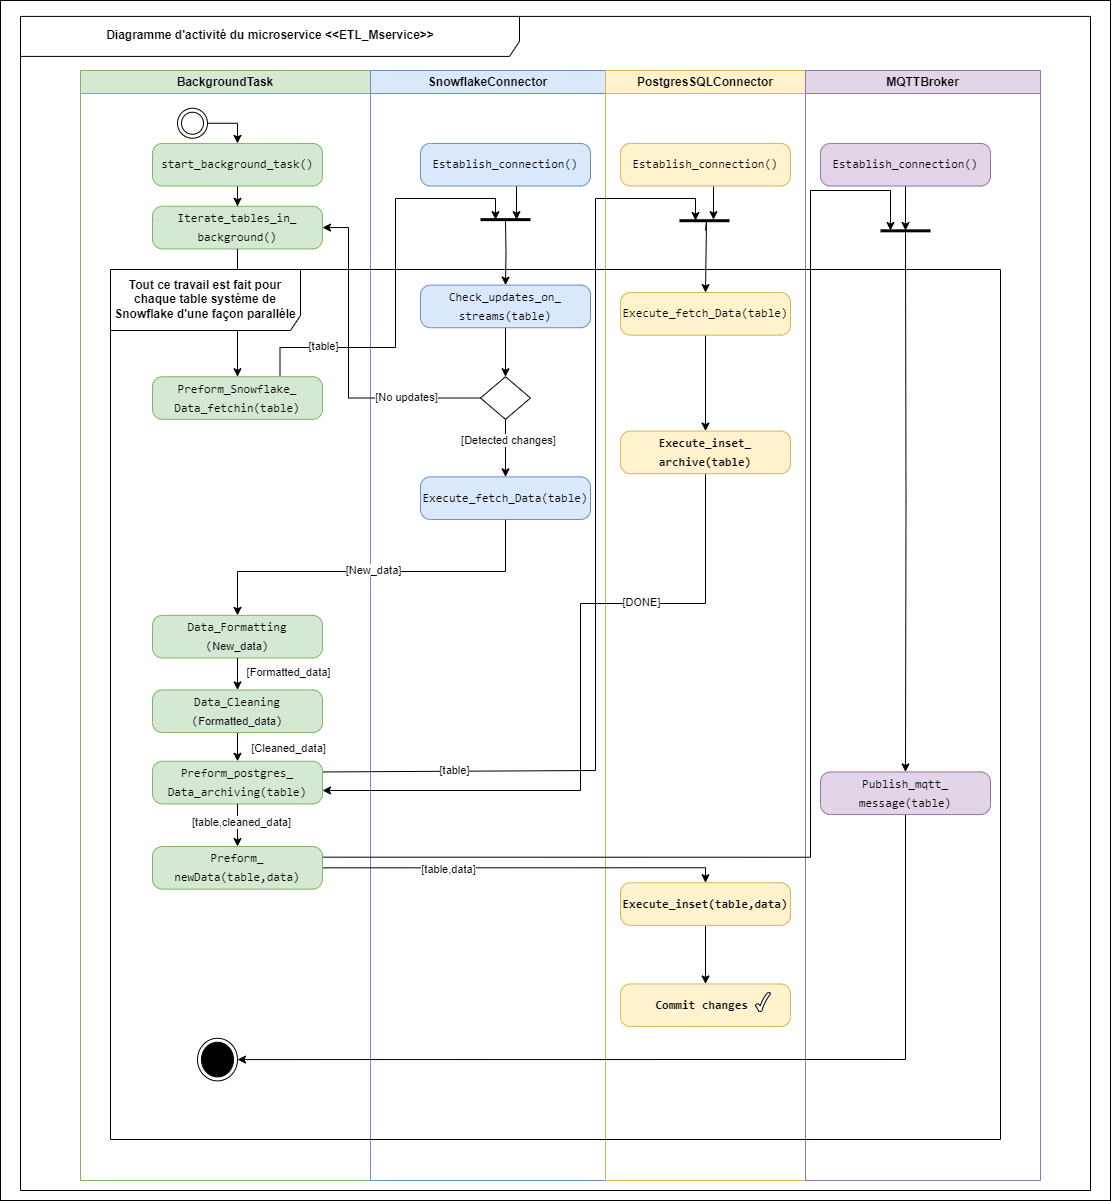
\includegraphics[width=1\linewidth, height=17cm]{img/conception/diag_act_1.png}
        \caption{Diagramme d'activité du cas d'utilisation <<Récupération des données >>}
            \label{fig :act}
        \end{figure}
    %fin
\par Le traitement du cas d'utilisation <<Récupération des données >> commence par l'appel la méthode \\ \hbox{\textbf{<<start\_background\_task()>>}}, qui est une tâche programmée automatiquement (cron job) chaque 24 ou 12 heurs selon la préférence de l'administrateur.
En lançant cette méthode, elle parcourt les tables du système Snowflake, dont nous voulons projeter, en utilisant la méthode \textbf{<<iterate\_tables\_in\_background()>>}.
\par À ce stade, le connecteur Snowflake établit une connexion avec le système Snowflake via la méthode \textbf{<<establish\_connection()>>}, 
qui à sa part connecte notre service avec le compte Snowflake dont nous souhaitons monitorer ces données plus tard.
\par Ensuite, le contrôleur système vérifie s'il y a des mises à jour sur les tables Snowflake en appelant la méthode \textbf{<<check\_updates\_on\_streams(tables)>>}. 
\par Si il y a des changements détectés, la méthode \textbf{<<execute\_fetch\_data(table)>>} est exécutée pour récupérer les nouvelles données de la table Snowflake.
\par Les nouvelles données récupérées sont ensuite transmises à l'étape de formatage des données \newline \textbf{<<Data\_Formatting()>>}, où elles sont mises en forme(typage, longeur, format etc.). 
Après cela, l'étape de nettoyage des données \textbf{<<Data\_Cleaning()>>} intervient pour préparer et nettoyer les données formatées. 
\par Postérieurement, l'étape d'archivage des données dans PostgreSQL \textbf{<<Preform\_Data\_archiving>>}, là où nous allons transformer les anciennes données de cette table vers une base de données d'archivage afin d'avoir toujours une traçabilité des données. 
\par Parallèlement, le connecteur PostgreSQL établit une connexion avec les base de données PostgreSQL, \textbf{monitoring\_db} et la base d'archive \textbf{backup\_db}, via la méthode \textbf{<<establish\_connection()>>}. 
tout en éxécutant la méthode \textbf{<<execute\_insert\_archive(table, data)>>}. 
\par Par la suite, le système déclanche la méthode \textbf{<<Preform\_newData(table,data)>>} pour insérer les nouveaux données nettoyées dans la base de données de monitoring. 
Après l'insertion des données, le microservice effectue un commit des changements dans la base de données.
\par il faut notez bien que, ce flux de travail ce repéte éventuellement pour chaque table, séparament ou/et séquentiellement pour les tables qui ont une relation entre eux, dans un \textbf{<<thread>>} à part.
\par Aprés la mise à jour de tout les tables, la tâche publie un message MQTT via la méthode \newline \textbf{<<publish\_mqtt\_message()>>} afin de notifier le systéme de l'ajout de nouvelles données. 
\par Cette approche garantit que toutes les étapes sont correctement coordonnées et que chaque composant est informé des mises à jour de manière efficace et en temps réel.
\par Enfin, le microservice ETL-service termine son traitement en attendant son prochain déclanchement.
\subsubsection{Diagrammme de séquence de cas d'utilisation <<Visualiser DAG>> :}
\par Un diagramme de séquence est un type de diagramme d'interaction, car il décrit comment et dans quel ordre plusieurs objets fonctionnent ensemble \cite{seq}.
\par Le diagramme de séquence de cas d'utilisation <<Visualiser DAG>> est représenté dans la figure \textbf{\ref{fig :seq1}} suivante :
    %code image
    \begin{figure}[H]
        \centering
        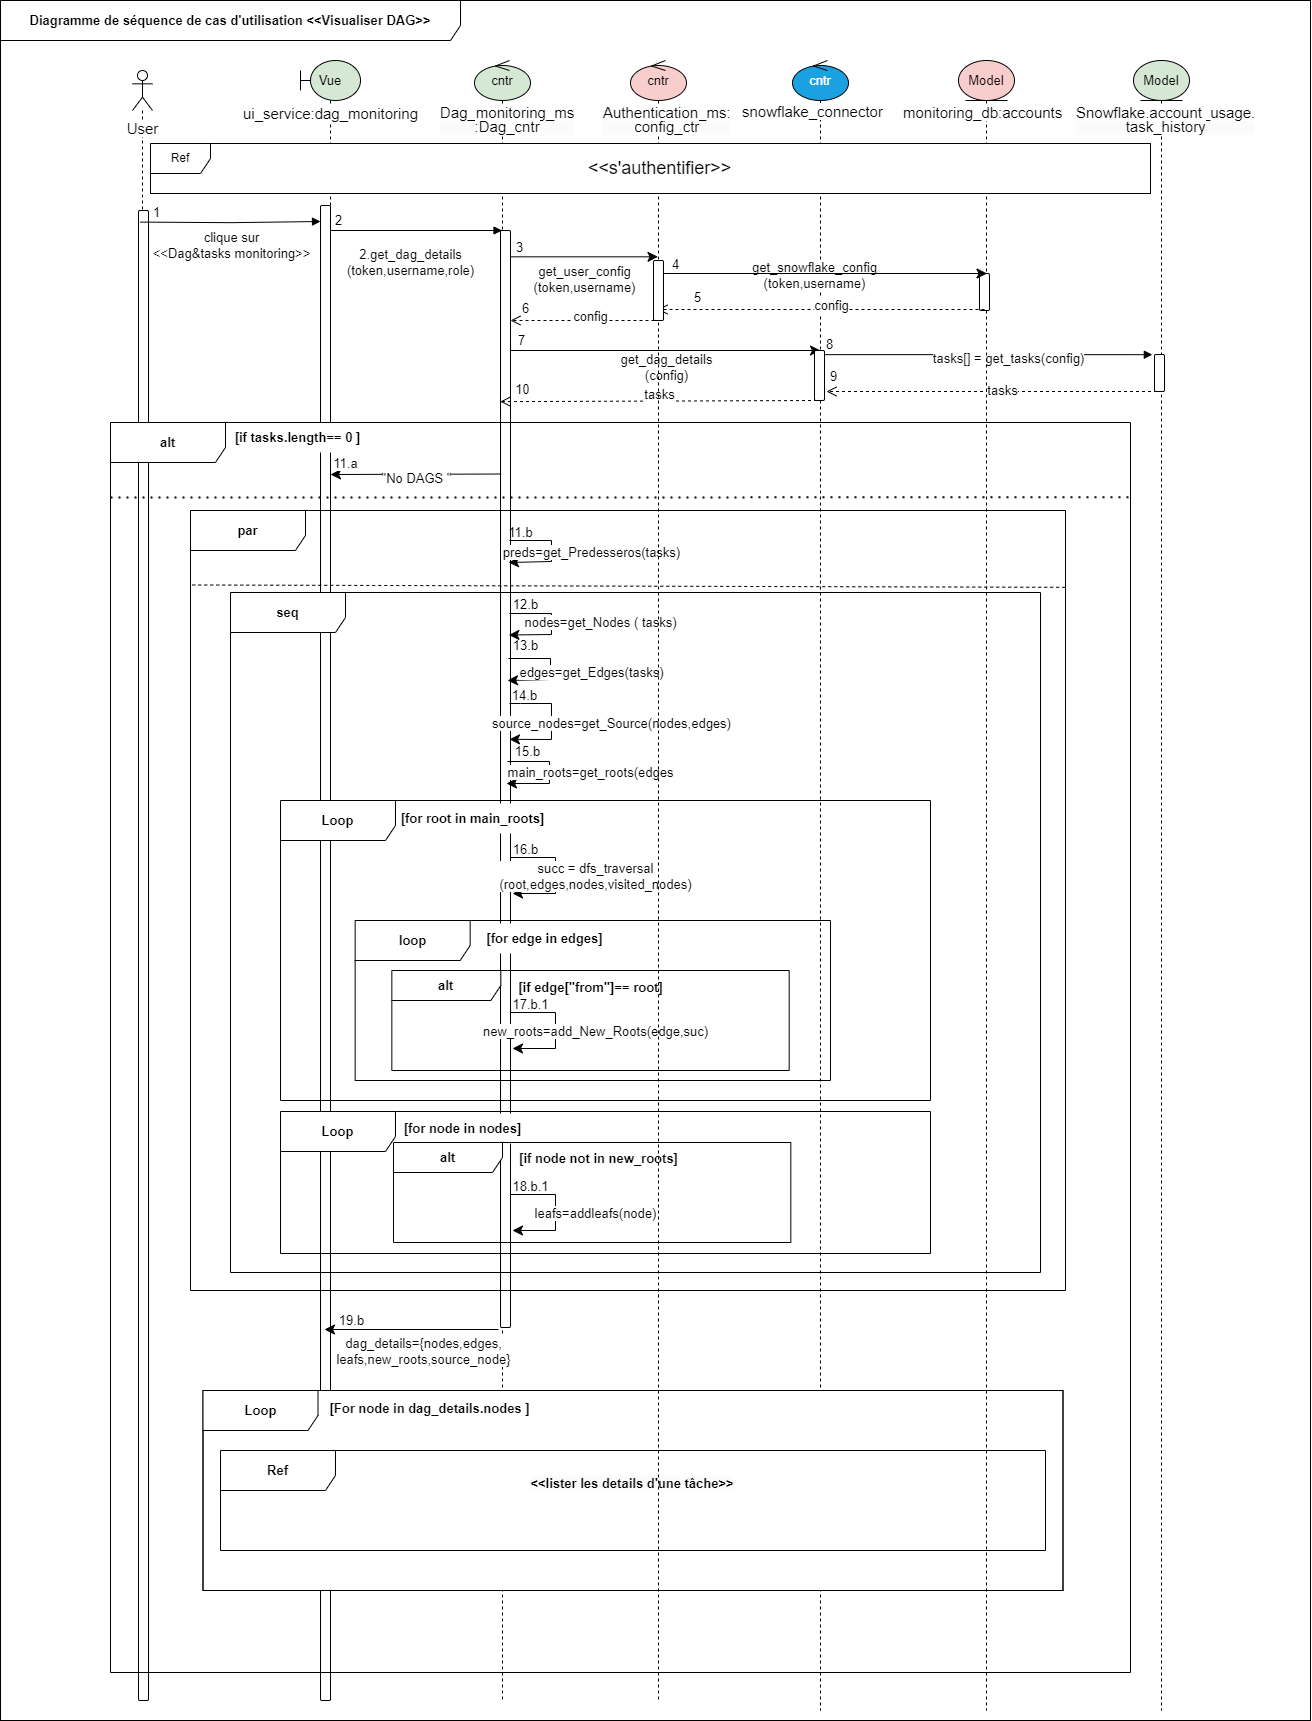
\includegraphics[width =1\linewidth, height=23.5cm]{img/conception/seq1.png}
        \caption{Diagrammme de séquence de cas d'utilisation <<Visualiser DAG>> }
            \label{fig :seq1}
    \end{figure}
    \par Ce diagramme de séquence décrit le cas d'utilisation \textbf{<<Visualiser le DAG>>} où 
    un utilisateur souhaite visualiser les détails du Directed Acyclic Graph (DAG) des tâches Snowflake en temps réel. \\
    \par Le traitement se lance lorsque l'utilisateur clique sur le bouton <<Task\&Dag Monitoring>> de l'interface, 
    cette action lance un appel au contrôleur du micro service <<DAG\&tasks\_monitoring>> pour récupérer les données spécifiques à chaque DAGs.
    Une fois l'appel est lancé, le contrôleur en question envoit à son tour une requête au micro-service d'authentification pour avoir les configurations de compte Snowflake assosiés au nom d'utilisateur avec la token d'autorisation.
    \par Le contrôleur snowflake config\_ctr du service d'authentification renvoit les configurations néssesaires au contrôleur principal.
    \par Lorsque les configurations sont retournées, le contrôleur de DAG\_monitoring fait appel au snowflake\_connector, qui est le point de communication direct entre l'application et Snowflake, pour accéder au compte Snowflake de l'utilisateur et récupérer la liste des tâches qui lui sont associées.
    \par le contrôleur snowflake\_ctr effectue les opérations nécessaires sur Snowflake et retourne la liste des tâches au DAG\_ctr :
    \begin{itemize}
        \item \textbf{Si [la longeur de la liste égal à 0];} le contrôleur DAG\_ctr renvoit un message au service du frontend en indiquant qu'il y a aucune DAG pour cette utilisateur,
        \item \textbf{Sinon;} \parindent=1.5em \par -le contrôleur DAG\_ctr commance le traitement sur les tâches retournées, en récupérant la liste des prédécesseurs de chaque tâches ;
       
        \parindent=1.5em \par -Parallèlement, dans un autre thread séparament, il recupére :les noeuds (nodes), les arêtes (edges), les noeuds sources (source\_nodes), les routes principales (main\_roots) ;
        \parindent=1.5em \par -Ensuite, pour chaque route il fait un parcours en profondeur (DFS\_transfersal) afin marquer les noeuds visités et collecter les successeurs ;
        \parindent=1.5em \par -Puis, il verife pour chaque arête, si l'arête part de la racine actuelle et si c'est le cas, il ajoute le noeud de destination au new\_roots qui sera l'ensemble des nouvelles racines pour la prochaine itération de la boucle principale ;
        \parindent=1.5em \par -Aprés tout cela, il parcourt tout les noeuds pour identifier les noeuds feuilles, ceux qui ne sont pas dans new\_root ;
        \parindent=1.5em \par -Finalement, il renvoit tout les informations traitées aux service frontend comme etant un objet JSON.
                
    \end{itemize}
    \par Enfin, le service frontend va lui même parcoure les noeudes de l'objet retourné, en dessinant le DAG finale en faisant appel au contrôleur Task\_details (cas d'utilisation <<lister les details d'une tâche>>) inclus du même service pour afficher en details chaque noeud du DAG.
    \par \textbf{NB :} Il faut bien préciser que le déclanchement de ce cas d'utilisation nécessite l'authentification de l'utilisateur et qu'il a les permissons et les rôles qui lui permet de visualiser les DAGs.
    \subsubsection{Diagramme de séquence du cas d'utilisation <<Lister les détaills d'une tâche>> :}
    \par La figure \textbf{\ref*{fig :seq2}} illustre le diagramme de séquence du cas d'utilisation <<Lister les détaills d'une tâche>> :

    \begin{figure}[H]
        \centering
        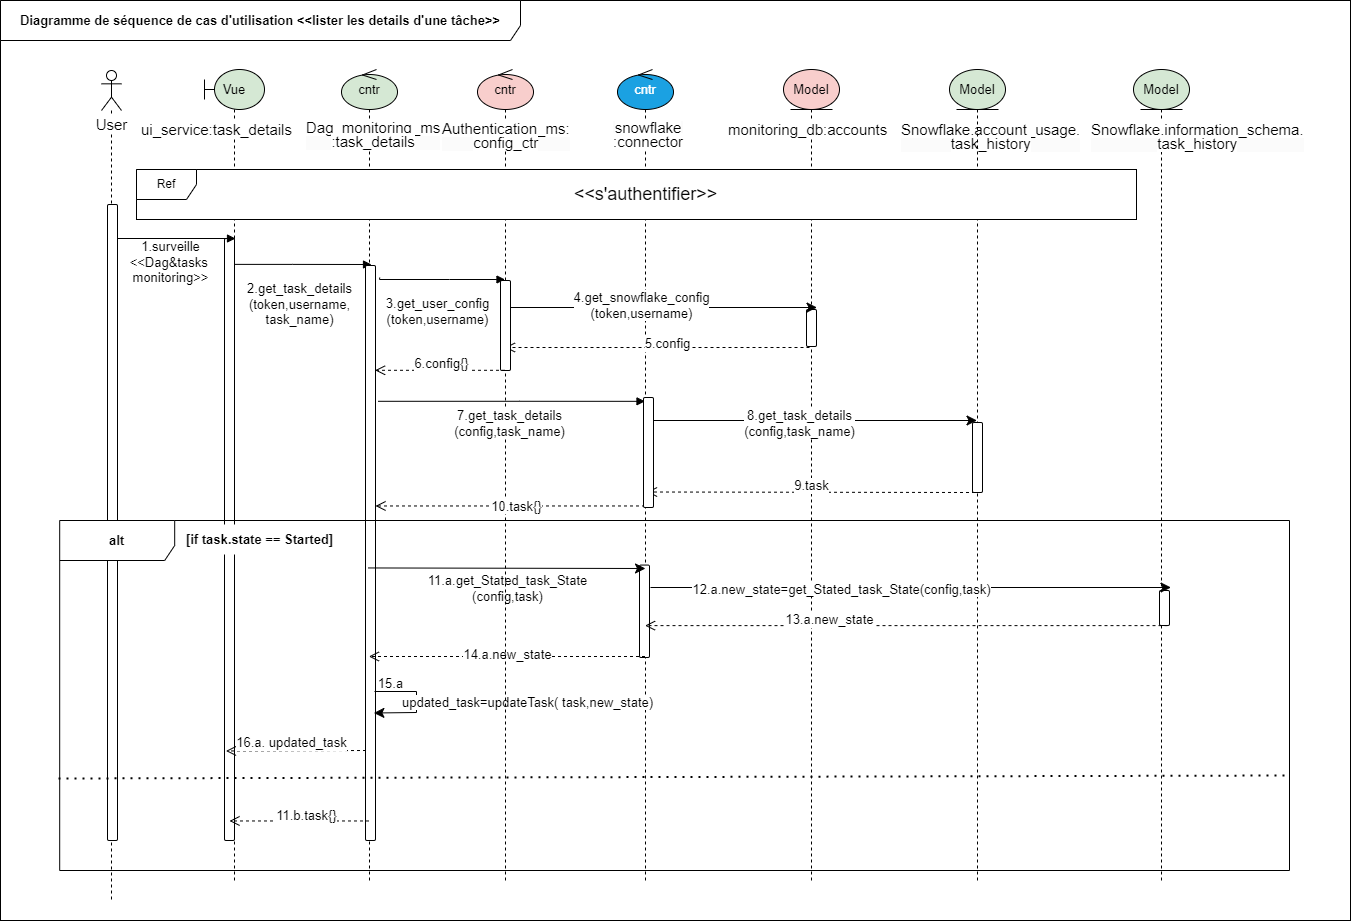
\includegraphics[width=1\linewidth ,height=17cm]{img/conception/seq2.png}
        \caption{Diagrammme de séquence de cas d'utilisation <<Lister les détaills d'une tâche>> }
        \label{fig :seq2}
    \end{figure}
    \par Pour Lister les details d'une tâche, et aprés avoir vérifier que l'utilisateur est authentifié, le service du frontend lance un appel au contrôleur task\_details 
    pour récupérer les données souhaitées. 
    \par En lançant cet contrôleur, il envoit à son tour une requête au micro-service d'authentification pour avoir les configurations de compte Snowflake assosiés au nom d'utilisateur avec la token d'autorization.
    \par Le contrôleur snowflake config\_ctr du service d'authentification renvoit les configurations néssesaires au contrôleur principal.
    \par Une fois les configurations sont retournées, le contrôleur de DAG\_monitoring fait appel au \par snowflake\_connector, qui est le point de communication direct entre l'application et Snowflake, 
    pour accéder au compte Snowflake de l'utilisateur et récupérer les détailles de tâche en question de la vue \textbf{Task\_History} du schéma système de snowflake \textbf{Account\_Ussage}, qui a des informations global sur les tâches.
    \par le contrôleur snowflake\_ctr effectue les opérations nécessaires sur Snowflake et retourne les détailles du task demandé sous le format JSON.
    \par Le contrôleur task\_details traite le résultat retourné; 
    \begin{itemize}
        \item \textbf{Si [L'état du tâche est <<Started>>] :} 
        \par - le contrôleur task\_details relance un autre appel au snowflake\_connector,
        \par - ce dernier il va accéder à nouveau à Snowflake mais cette fois si il va opérer la vue \textbf{Task\_History} du schéma \textbf{Information\_schema} de Snowflake, qui est la vue qui a les informations sur les tâches commencées, pour récupérer l'êtat de cette tâche en temps rélle qui peut être ( plannifiée, entrain de s'éxécuter ou échouée),
        \par - une fois le nouveau état est retourner task\_details met à jour les données en modifiant l'état <<Started>> par le nouveau ètat du tâche et l'envoyer au service du frontend en fomat JSON.
        \item \textbf{Sinon [L'état sera <<suspended>>] :} le controleur va retourner directement les données du tâche au service de frontend sans faire aucune modification.
    \end{itemize}

    \subsubsection{Diagramme de séquence du cas d'utilisation <<Créer un compte>> :}
    \par La figure \textbf{\ref*{fig :seq3}} illustre le diagramme de séquence du cas d'utilisation <<Créer un compte>> :
    \begin{figure}[H]
        \centering
        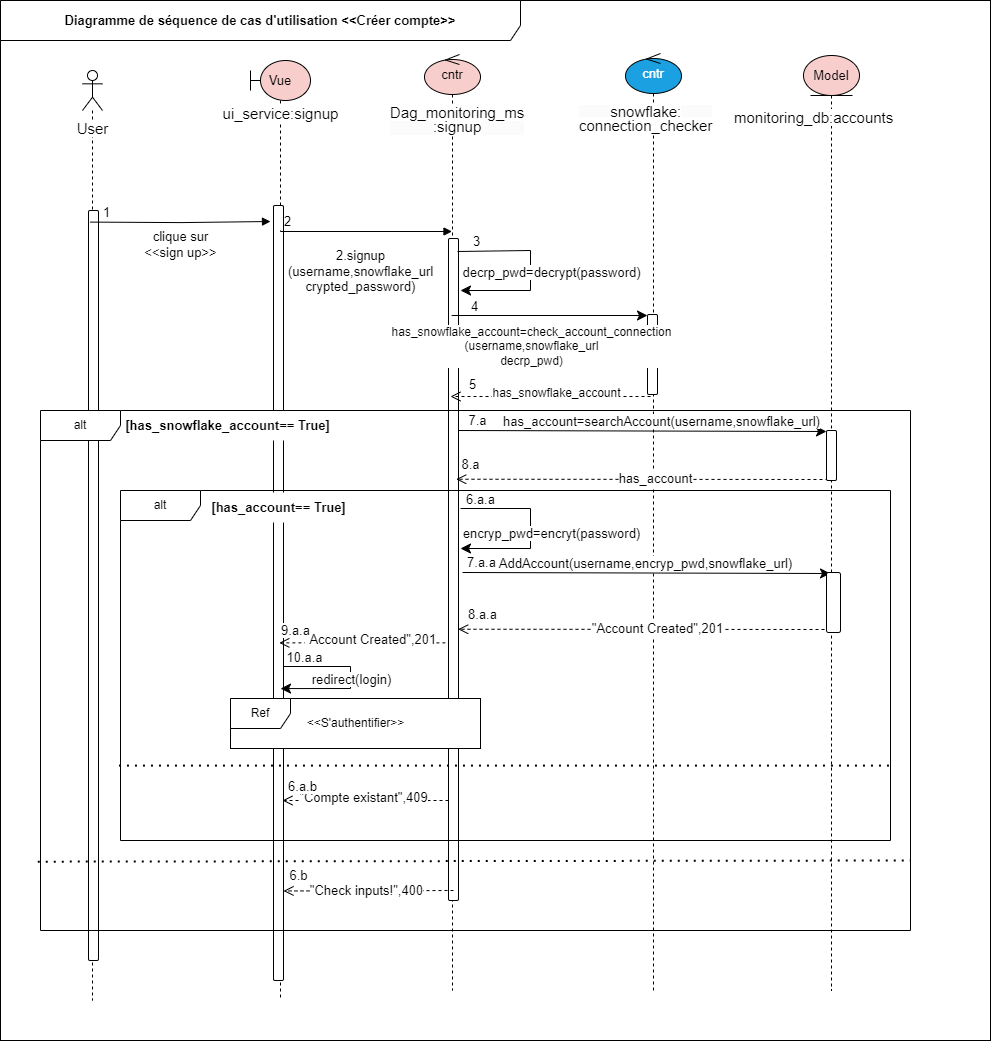
\includegraphics[height=17cm]{img/conception/signup.png}
        \caption{Diagrammme de séquence de cas d'utilisation <<Créer un compte>> }
        \label{fig :seq3}
    \end{figure}
    \par Afin de pouvoir s'inscrire dans <<Snowflake Monitoring Application>>, l'utilisateur accéde à l'interface de création de compte de l'application en saisisant son nom d'utilisateur, mot de passe, 
    ainsi que l'URL d'accés à son compte Snowflake.
    \par En cliquant sur <<signup>>, le contrôleur signup\_ctr récupére les données saisies du frontend et décrypte le mot de passe.
    \par Ensuite, il emettre un appel au contrôleur de snowflake pour que ce dernier vérifie l'existance de ce compte dans Snowflake en retournant une réponse vers le contrôleur principal. 
    \begin{itemize}
        \item \textbf{[has\_snowflake\_account == True]} :
       \par -le contrôleur lance une recherche dans la table de monitoring\_DB \textbf{accounts}
       \par -\textbf{si [has\_account == True]}, le contrôleur renvoit une erreur au frontend.
       \par -\textbf{sinon}, le contrôleur va encrypter le mot de passe et crée un compte dans la table \textbf{accounts} avec les données saisies.
       \par Enfin, il va renvoyer un message de succéss au frontend qui va à son tour rediger l'utilisateur vers la page de l'authentification. 
       \item \textbf{[Sinon]} : 
       \par -Le contrôleur renvoie un message d'erreur au frontend en indiquant que les données saisies n'appartiennent à aucun compte Snowflake.
    \end{itemize}
    \subsubsection{Diagramme de séquence du cas d'utilisation <<S'authentifier>> :}
    \par La figure \textbf{\ref*{fig :seq4}} illustre le diagramme de séquence du cas d'utilisation <<S'authentifier>> :

    \begin{figure}[H]
        \centering
        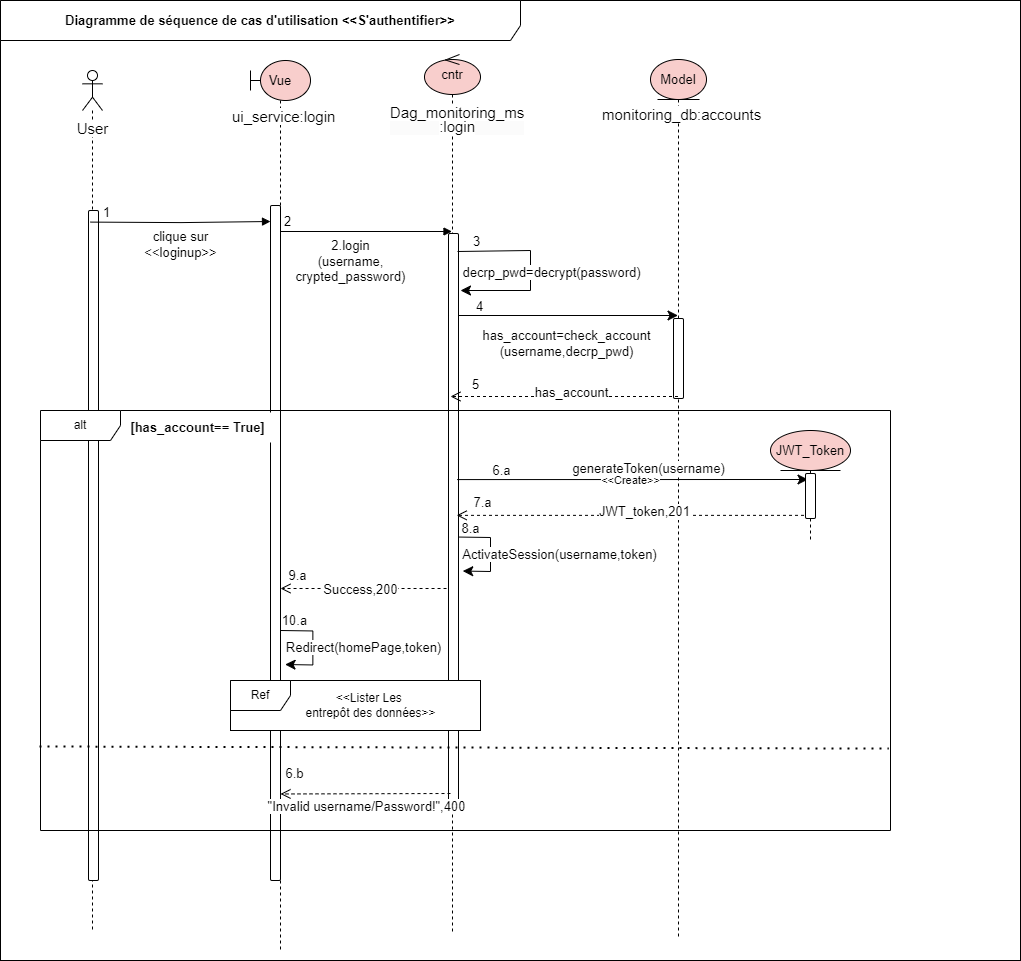
\includegraphics[ height=12cm]{img/conception/login.png}
        \caption{Diagrammme de séquence de cas d'utilisation <<S'authentifier>> }
        \label{fig :seq4}
    \end{figure}
    \par Pour accéder à l'application, l'utilisateur accéde à l'interface de <<login>> en saisissant les données d'authentification (nom d'utilisateur, mot de passe).
    \par En cliquant sur <<login>>, le contrôleur login\_ctr récupére les données saisies du frontend et décrypte le mot de passe saisie. 
    \par Ensuite, il lance une recherche dans la table \textbf{Accounts} pour vérifier l'existance du compte; 
    \begin{itemize}
        \item \textbf{[Has\_account == True]} : cela signifie que le compte existe déjà, et là le contrôleur crée une instance de l'objet \textbf{JWT Token}, qui est le moyen d'accés à toutes les informations et parties de l'application.
         Une fois l'instance est créée et retournée le contrôleur active la session de connexion de l'utilisateur et retourne la token ainsi que un message de succés au frontend.
        \par Finalement, le frontend redirige l'utilisateur vers la page d'acceuil de l'application.
        \item \textbf{[Sinon (compte inexistant)]} : le contrôleur renvoit un message d'erreur vers le frontend en indiquant que les données saisies sont invalides.
    \end{itemize}
    \section*{Conclusion}
\addcontentsline{toc}{section}{Conclusion }
\par Ce chapitre a établi les bases pour la mise en œuvre technique de notre projet. Les choix architecturaux et conceptuels se sont avérés essentiels pour assurer la stabilité et la performance de notre solution. Dans le prochain chapitre, nous plongerons dans la réalisation concrète de notre projet.